\documentclass[tikz, border=5, convert]{standalone}
\usepackage{pgfplots}
\usepgfplotslibrary{patchplots}
\begin{document}
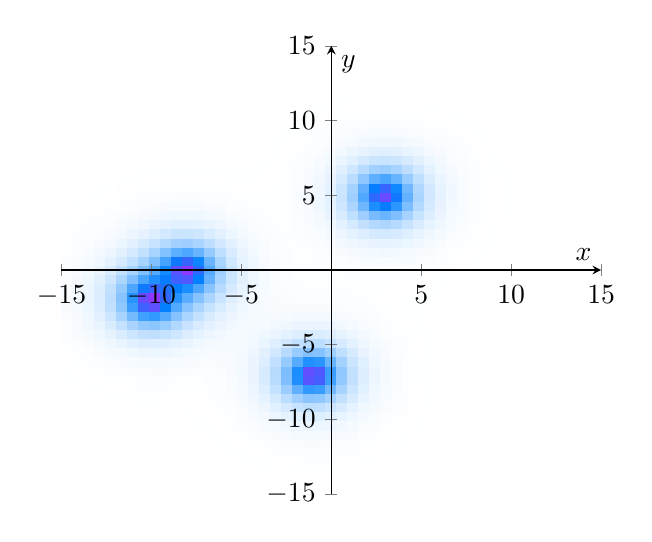
\begin{tikzpicture}[>=stealth]

\begin{axis}[view={0}{90},axis lines=middle, xlabel=$x$, ylabel=$y$]
	\pgfplotsset{colormap/cool}
	\addplot3 [surf, shader= flat, domain=-15:15, samples=50] {
		exp(-sqrt((x+8)^2+(y-0)^2))+
		exp(-sqrt((x-3)^2+(y-5)^2))+
		exp(-sqrt((x+1)^2+(y+7)^2))+
		exp(-sqrt((x+10)^2+(y+2)^2))};

%    \addplot [scatter, only marks] table[x=x, y=y]{
%    x y
%    -0.8 0
%    0.3 0.5
%    -0.1 -0.7
%    -1 -0.2
%    };
\end{axis}

	
\end{tikzpicture}
	
\end{document}
